% Autor: Leonhard Segger, Alexander Neuwirth
% Datum: 2017-10-30
\documentclass[
	% Papierformat
	a4paper,
	% Schriftgröße (beliebige Größen mit „fontsize=Xpt“)
	12pt,
	% Schreibt die Papiergröße korrekt ins Ausgabedokument
	pagesize,
	% Sprache für z.B. Babel
	ngerman
]{scrartcl}

% Achtung: Die Reihenfolge der Pakete kann (leider) wichtig sein!
% Insbesondere sollten (so wie hier) babel, fontenc und inputenc (in dieser
% Reihenfolge) als Erstes und hyperref und cleveref (Reihenfolge auch hier
% beachten) als Letztes geladen werden!

% Silbentrennung etc.; Sprache wird durch Option bei \documentclass festgelegt
\usepackage{babel}
% Verwendung der Zeichentabelle T1 (Sonderzeichen etc.)
\usepackage[T1]{fontenc}
% Legt die Zeichenkodierung der Eingabedatei fest, z.B. UTF-8
\usepackage[utf8]{inputenc}
% Schriftart
\usepackage{lmodern}
% Zusätzliche Sonderzeichen
\usepackage{textcomp}

% Mathepaket (intlimits: Grenzen über/unter Integralzeichen)
\usepackage[intlimits]{amsmath}
% Ermöglicht die Nutzung von \SI{Zahl}{Einheit} u.a.
\usepackage{siunitx}
% Zum flexiblen Einbinden von Grafiken (\includegraphics)
\usepackage{graphicx}
% Abbildungen im Fließtext
\usepackage{wrapfig}
% Abbildungen nebeneinander (subfigure, subtable)
\usepackage{subcaption}
% Funktionen für Anführungszeichen
\usepackage{csquotes}
% Zitieren, Bibliographie
\usepackage{biblatex}


% Zur Darstellung von Webadressen
\usepackage{url}
%chemische Formeln
\usepackage[version=4]{mhchem}
% siunitx: Deutsche Ausgabe, Messfehler getrennt mit ± ausgeben
\usepackage{floatrow}
\usepackage{float}
\floatsetup[table]{capposition=top}
% Verlinkt Textstellen im PDF-Dokument
\usepackage[unicode]{hyperref}
% "Schlaue" Referenzen (nach hyperref laden!)
\usepackage{cleveref}
\sisetup{
	locale=DE,
	separate-uncertainty
}
%\bibliography{6Mi_M3_29-11-2017_References}

\begin{document}
	
	\begin{titlepage}
		\centering
		{\scshape\LARGE Versuchsbericht zu \par}
		\vspace{1cm}
		{\scshape\huge E3 - Elektrische Resonanz \par} 
		\vspace{2.5cm}
		{\LARGE Gruppe 6Mi \par}
		\vspace{0.5cm}
		
		{\large Alexander Neuwirth (E-Mail: a\_neuw01@wwu.de) \par}
		{\large Leonhard Segger (E-Mail: l\_segg03@uni-muenster.de) \par}
		\vfill
		
		durchgeführt am 17.01.2018\par
		betreut von\par
		{\large Wladislaw Hartmann} %TODO Ich hoffe, das ist der richtige
		
		\vfill
		
		{\large \today\par}
	\end{titlepage}
	\tableofcontents
	\newpage

	%TODO mehr TODO in Default	

	\section{Kurzfassung}
	%TODO Hypothese	und deren Ergebnis
	%TODO Ergebnisse, auch Zahlen, mindestens wenn's halbwegs Sinn ergibt
	%TODO Was wurde gemacht
	In diesem Versuch wurde das elektrische Resonanzverhalten von einem Serienresonanzkreis und einem Parallelresonanzkreis untersucht.
	Dazu wurden die entsprechenden Schwingkreise durch einem Funktiongenerator zum Schwingen angeregt.
	Mit einem Multimeter wurde die Spannung über einen \SI{10}{\Omega} Widerstand in Abhängigkeit von der Kapazität des Kondensators bestimmt, da ein Variieren der Frequenz des Stroms weniger praktikabel ist, um die Resonanz des Schwingkreises quantisieren.  %TODO effektive Stromstärke und Spannung??
	Je Resonanzkreis wurden für 3 unterschiedliche  Widerstände und jeweils 20 verschiedenen, um den Resonanzfall gehäufte, Kapazitäten die Stromstärke erfasst.
	Der Innenwiderstand der jeweiligen Spulen im Schwingkreis lässt sich aus der aufgenommenen Resonanzkurve bestimmen.
	Die Hypothese, dass dieser dem direkt durch das Multimeter bestimmen Innenwiderstand entsprechen muss, wurde im folgenden überprüft. %TODO behandeln weil net schon wieder untersuchen.
	%ERGEBNISSE

	%TODO aufgenommene Werte vergleichen was produziert wurde.

	\section{Methoden}
	%TODO Bilder von der Website klauen
	Als Erstes wurde eine Reihenschwingkreis aufgebaut (\cref{serieAufbau}).
	Mit dem Multimeter wurde die Spannung über den \SI{10}{\Omega} Widerstand gemessen, sodass sich daraus die Strokstärke bestimmen lässt.
	Mit dem Funktiongenerator und dem Oszilloskop wurde die Frequenz des Wechselstorms auf \SI{1}{kHz} und eine Peak-Peak-Spannung von \SI{4}{V}.

	Für 3 Widerstände (\SI{200}{\Omega}, \SI{500}{\Omega} und \SI{0}{\Omega}) wurden die am Multimeter gemessenen Spannungen in Abhängigkeit von der eingestellten Kapazität aufgenommen .
	Diese Kapazität wurde in kleinen Schritten nahe dem Resonanzfall, also maximaler Spannung, abgetastet.
	Die im Resonanzfall angezeigte Peak-Peak-Spannung am Oszilloskop wurde ebenfalls erfasst.
	Zuletzt wurde der Widerstand der Spule mit dem Multimeter gemessen.

	Die Untersuchung des Parrallelschwingkreises erfolgte analog (\cref{paralleAufbau}), jedoch mit einer anderen Spule, anderen Widerständen (\SI{2}{k\Omega}, \SI{10}{k\Omega} und $\infty$ \SI{}{k\Omega}) und einer Peak-Peak-Spannung von \SI{10}{V}.
	Ein weiterer Unterschied der Schwingkreise ist, dass im Parallelschwingkreis der Resonanzfall bei minimaler Spannung auftritt.
	\begin{figure}[H]
		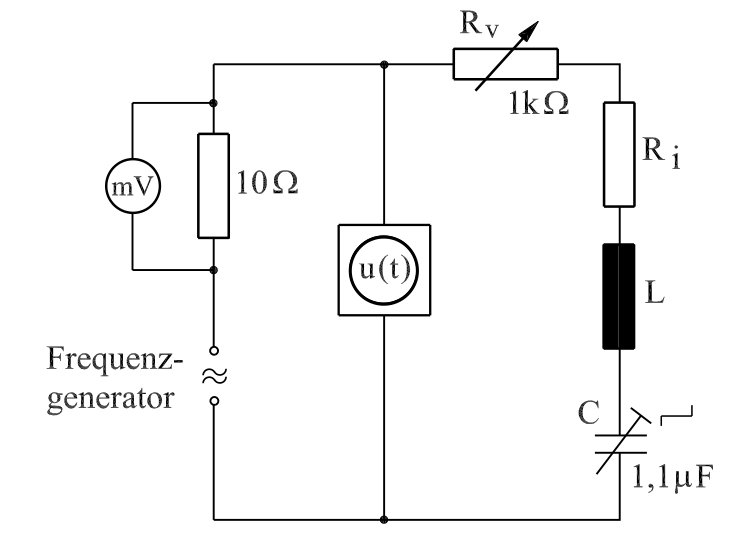
\includegraphics[width=0.4\textwidth]{serieAufbau}
		\centering
		\caption{Experimenteller Aufbau des Serienresonanzkreises.} %TODO cref/literatur von learnweb
		\label{serieAufbau}
		\centering
	\end{figure} 
		\begin{figure}[H]
		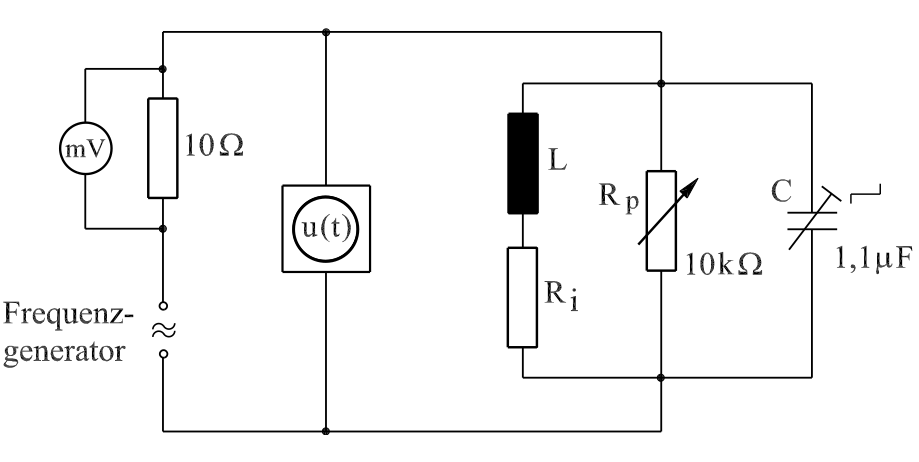
\includegraphics[width=0.4\textwidth]{parallelAufbau}
		\centering
		\caption{Experimenteller Aufbau des Parallelresonanzkreises.} %TODO KReis oder Kreises
		\label{parallelAufbau}
		\centering
	\end{figure}

	

	\section{Ergebnisse und Diskussion}
	%TODO Datenanalyse -> Überschrift?
	%TODO Unsicherheiten
	

	\subsection{Beobachtung}

	\subsection{Diskussion}
	%TODO Bezug/Nutzten oder sonst was
	%TODO auch hier die Hypothese wiederholen
	
	\section{Schlussfolgerung}
	%TODO Rückgriff auf Hypothese und drittes Nennen dieser
	
	%TODO Quellen zitieren, Websiten mit Zugriffsdatum
	%TODO Verweise auf das Laborbuch (sind erlaubt)
	%TODO Tabelle + Bilder mit Beschriftung
	%\printbibliography
\end{document}
